\documentclass[a4paper]{article}

\usepackage[italian]{babel}
\usepackage[T1]{fontenc}
\usepackage[utf8]{inputenc}
\usepackage{graphicx}
\usepackage[margin=1in]{geometry}
\usepackage{makecell}

\usepackage[table]{xcolor}

\usepackage{setspace}

\usepackage{tabularx} 

\usepackage{hyperref}
\usepackage{array}

\usepackage{fancyhdr}


\makeindex

\usepackage{hyperref}

\usepackage{float}
\makeindex

\title{
	\textbf{BORA BORA FITNESS CLUB}\\
	\large Relazione di progetto di Tecnologie Web
}
\date{Anno 2021 - 2022}

\begin{document}
	\maketitle

	\begin{center}
		\begin{tabular}{c|l l}
			\textbf{Componenti}	& Adnan Latif Gazi			& 1224442\\
								& Alberto Lazari			& 1216747\\
								& Marco Andrea Limongelli	& 1225415\\
								& Francesco Protopapa		& 1221598\\
		\end{tabular}
	\end{center}

	\begin{center}
		\begin{tabular}{|l|l|l|}
			\hline
			\textbf{Tipologia di utente}	& \textbf{Username}	& \textbf{Password}\\
			\hline
			Utente generico					& user				& user\\
			\hline
			Utente amministratore			& admin				& admin\\
			\hline
		\end{tabular}
	\end{center}

	% indice
	\renewcommand{\contentsname}{Indice}
	\tableofcontents
	\pagebreak

	\section{Introduzione}
	\subsection{Abstract}
	Il progetto Bora Bora Fitness Club, svolto come finalità del corso di Tecnologie Web nell'anno accademico 2021-2022, si propone di implementare un sito Internet per la gestione delle attività relativa ad una palestra. Il nome è ottenuto unendo i titoli dell'isola della polinesia francese di Bora Bora, in cui sorge l'attività, con una classica e indicativa denominazione delle palestre (Fitness Club). Per conseguire lo scopo, la natura del sito è fortemente interattiva, ma unisce anche una sostanziosa parte per la presentazione dell'impresa. Per i visitatori è infatti possibile accedere al proprio account, grazie al quale gestire le proprie attività di palestra. Nonostante ciò l'autenticazione non è obbligatoria: il visitatore ha comunque a disposizione tutte le funzionalità informative. Il sito è stato sviluppato con l'intenzione di essere poi pubblicato su Internet, dunque si è data molta importanza alla sua usabilità, rispettando gli standard W3C, la separazione tra struttura, presentazione, comportamento e le regole di accessibilità richieste.

	\subsection{Analisi dell'utenza}
	Il sito web si rivolge prevalentemente ad un pubblico di abitanti o visitatori dell'isola che intendono allenarsi nella sua unica palestra disponibile. Sebbene in minima parte, viene anche utilizzato dai gestori della palestra e una parte dei clienti degli alberghi convenzionati, che, pagando la quota una tantum di iscrizione all'albergo, hanno libero accesso alla palestra fintantoché pernottano nel relativo resort. Raccoglie pertanto una clientela relativamente giovane e al passo con la tecnologia. Il sito risulta essere ottimizzato per la visualizzazione da telefono, in quanto è stato appurato che la maggior parte degli utenti salvino i propri allenamenti nel sito, e una volta arrivati in palestra si allenino seguendo la scheda degli esercizi direttamente dal telefono. Viene prevista, inoltre, la presenza di una piccola parte della clientela non aggiornata con le ultime tecnologie e non in grado di comprendere o utilizzare le funzionalità più moderne: a tal proposito il sito è stato realizzato ponendo massima attenzione all'usabilità per ogni tipo di tecnologia e utente. L'utenza target del sito si divide in 3 gruppi, una volta che visitano il sito:
	\begin{itemize}
		\item Admin: amministra sugli utenti e le loro attività in modo da regolare il corretto funzionamento del sito.
		\item Utente registrato: usufruisce delle funzionalità di gestione delle proprie attività in modo da godere della più ampia esperienza di palestra.
		\item Utente non registrato: ricerca informazioni da una panoramica della palestra al fine di valutare il suo interesse per la palestra.
		
	\end{itemize}

	\section{Progettazione}

	\subsection{Scenari d'uso}

	\subsection{Struttura del sito}
	\begin{figure}
		\centering
		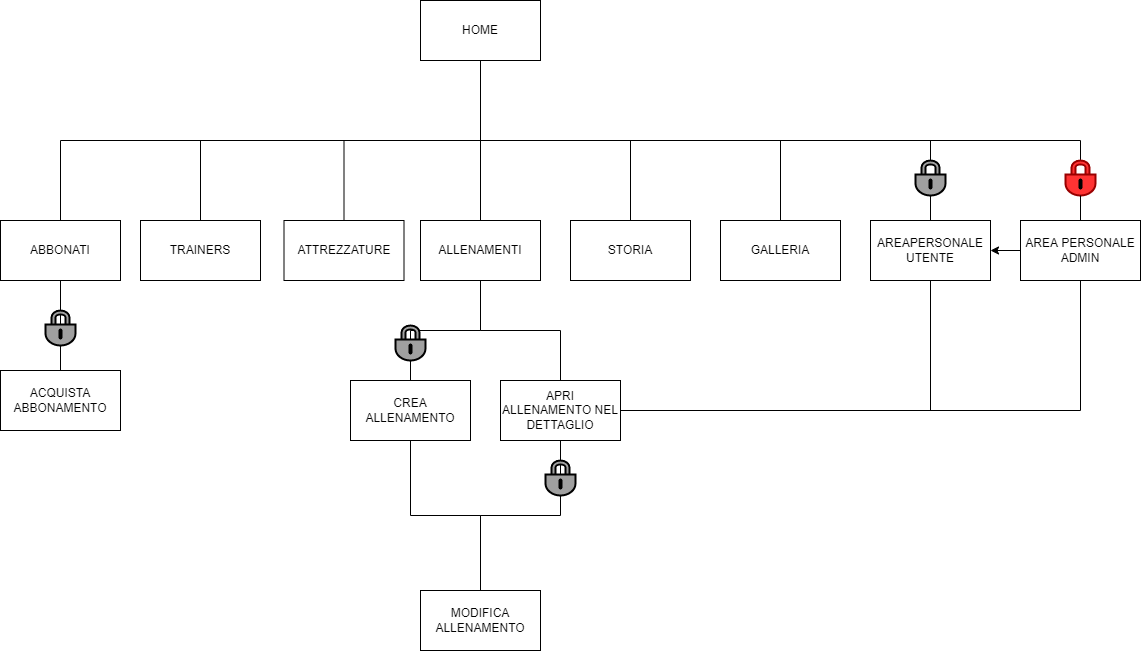
\includegraphics[scale=0.3]{immagini/mappa sito.drawio.png} 
	\end{figure}
	\begin{itemize}
		\item Home: è la prima pagina che viene visualizzata quando un utente visita il sito e ha lo scopo di far capire all'utente cosa può fare all'interno del sito. La pagina mostra le informazioni più importanti sulla palestra (come raggiungerci, orari di apertura, ecc.) e presenta una sezione che ha lo scopo di convincere l'utente ad iscriversi ad essa. È inoltre presente un link che porta alle proprie schede di allenamento il quale è una delle prime informazioni che vengono visualizzate nel layout mobile, questo per facilitare la navigazione agli utenti che vogliono consultare la propria scheda di allenamento dal telefono mentre sono in palestra.
		\item Abbonati: in questa pagina vengono illustrati i diversi tipi di abbonamento disponibili, da questa pagina è inoltre possibile accedere alla pagina di acquisto abbonamento.
		\item Acquista abbonamento: questa pagina accessibile solo agli utenti autenticati permette di scegliere una tipologia di abbonamento ed acquistarla, una volta effettuato l'acquisto l'utente verrà reindirizzato alla sua area personale.
		\item Trainers: questa pagina illustra i personal trainer che lavorano all'interno della palestra, ad ogni personal trainer è associato nome, età, una citazione, una descrizione, i suoi corsi e le sue specializzazioni.
		\item Attrezzature: in questa pagina sono presenti le foto di tutte le macchine e gli attrezzi presenti nella palestra con la relativa descrizione.
		\item Allenamenti: all'interno di questa pagina è possibile consultare le informazioni principali delle schede di allenamento create dagli utenti. Ogni tipologia di utente potrà consultare un allenamento nel dettaglio tramite l'apposito link, mentre solo gli utenti autenticati possono seguire gli allenamenti di altri utenti, creare un nuovo allenamento, modificare ed eliminare i propri allenamenti. Gli admin possono modificare ed eliminare gli allenamenti di tutti gli utenti.
		\item Crea allenamento: questa pagina accessibile solo agli utenti autenticati presenta una form per la creazione di un allenamento, se la pagina è visualizzata da un admin offre la possibilità di assegnare l'allenamento ad un utente specifico.
		\item Dettagli allenamento: all'interno di questa pagina è possibile visualizzare nel dettaglio un allenamento e offre anche la possibilità di stamparlo. La pagina è visitabile anche da utenti non autenticati.
		\item Modifica allenamento: questa pagina permette di modificare un allenamento creato da un utente, aggiungendo o eliminando esercizi. È visitabile solamente dall'utente specifico che ha creato quell'allenamento specifico e da un admin.
		\item Storia: questa pagina illustra la storia della palestra a partire da quando è stata fondata fino al giorno d'oggi
		\item Galleria: in questa pagina sono presenti le fotografie della palestra raggruppate in base alle diverse zone.
		\item Area personale utente: questa pagina accessibile solo agli utenti autenticati permette di visualizzare le proprie informazioni personali e modificarle, è inoltre possibile visualizzare le informazioni relative al proprio abbonamento e alle schede di allenamento create e seguite. È infine possibile effettuare il logout.
		\item Area personale admin: questa pagina accessibile solo agli admin offre le stesse funzionalità dell'area personale utente con l'aggiunta della gestione utenti (che non siano a loro volta degli amministratori) la quale permette di cercare o eliminare degli utenti o accedere alla loro area personale per visualizzare o modificare i dati relativi ai loro dati personali o relativi all'abbonamento e di visualizzare gli allenamenti seguiti e creati dall'utente.
		\item 404: questa pagina viene visualizzata solo in caso in cui una risorsa non venga trovata a causa di un errore di ricerca da parte dell'utente. Sfrutta una emotional design consona al dominio del sito per fornire consigli utili per risolvere il problema e permette di essere reindirizzato verso le altre pagine del sito, in modo da poter cercare nuovamente il contenuto desiderato.
		\item 500:
	\end{itemize}

	\section{Realizzazione}

	\subsection{Linguaggi}
	\begin{itemize}
		\item HTML5: abbiamo deciso di utilizzare lo standard HTML5 dato che secondo la nostra analisi dell'utenza, quasi tutti i visitatori del sito disporranno di dispositivi in grado di supportare questo standard. HTML5 ci permette di descrivere meglio la struttura della pagina con tag come article, header, footer, nav e altri. Inoltre ci è molto utile per alcune form dove al tag input vengono utilizzati i valori number, email, tel, date e time per l'attributo type;
		\item CSS3: è stato deciso di utilizzare lo standard css3 per facilitare la parte responsive del sito tramite l'utilizzo di flex e grid, inoltre i colori utilizzati dal sito sono salvati tramite variabili per facilitare la modifica e l'utilizzo della dark-mode;
		\item JavaScript: utilizzato per la validazione delle form lato client, l'implementazione della dark-mode e altre piccole features volte a migliorare la user experience. Non è stata utilizzata alcuna libreria esterna;
		\item PHP: utilizzato per la realizzazione di pagine web dinamiche, per le interazioni col database e la validazione delle form lato server;
		\item SQL: usato MySQL (MariaDB). Utilizzato per la creazione del database e per effettuare le query di ricerca per generare nelle pagine dinamiche in PHP.
	\end{itemize}

	\subsection{Strumenti}
	\begin{itemize}
		\item GitHub: strumento fondamentale per la collaborazione asincrona allo sviluppo del progetto;
		\item Chrome
		\item Firefox
		\item Xampp: software utilizzato per creare un web hosting locale che ci ha permesso di testare il sito anche da smartphone e tablet;
		\item https://webaim.org/resources/contrastchecker/ strumento utilizzato per la verifica del contrasto tra i colori presenti nel nostro sito;
		\item https://tools.pingdom.com/ strumento utilizzato per calcorare il peso delle pagine del sito.
		\item https://validator.w3.org per la validazione del codice HTML5
		\item https://jigsaw.w3.org/css-validator/ per la validazione del codice CSS
	\end{itemize}

	\section{Accessibilità}
	Per mantenere un alto livello di accessibilità ci siamo attenuti allo standard WCAG 2.0 (https://www.w3.org/Translations/WCAG20-it/)

	\subsection{Separazione tra comportamento, struttura e presentazione}
	Per migliorare l'accessibilità per gli utenti con differenti disabilità e per un miglior posizionamento nei motori di ricerca, abbiamo mantenuto una netta separazione tra comportamento, struttura e presentazione. Per quanto riguarda la struttura abbiamo utilizzato documenti HTML5, i quali sono stati stilizzati utilizzando documenti CSS esterni. Per il comportamento invece è stato utilizzato un documento Javascript esterno. Nel codice HTML non abbiamo inserito attributi relativi ad eventi Javascript in modo tale da separare completamente struttura da comportamento. Proprio per questo motivo è il codice Javascript a specificare gli eventi per ogni elemento HTML. Tutto il codice è stato scritto seguendo le raccomandazioni W3C, evitando l'utilizzo di tag e attributi deprecati, accertando la validità tramite l'utilizzo dei validatori.

	\subsection{WAI-ARIA}
	Per garantire l'accessibilità abbiamo deciso di utilizzare la specifica WAI-ARIA prodotta da W3C, che definisce un insieme di attributi HTML addizionali che possono essere applicati ai vari elementi per fornire maggior valore semantico e aumentare l'accessibilità. In particolare abbiamo utilizzato gli aria-label in quelle situazioni in cui non era presente testo, come per esempio il simbolo nel menù contenente il link per andare nell'area personale e nel footer nelle varie immagini utilizzate per le informazioni di contatto. Abbiamo inoltre utilizzato l'attributo aria-label anche sul breadcrumb per indicare che il contenuto di quel tag <nav> indica la posizione dell'utente all'interno del sito. Sempre riguardo alla navigazione, in ogni pagina abbiamo predisposto un link nascosto agli utenti ma visibile agli screen reader per saltare la lettura delle varie voci del menu e andare direttamente al contenuto della pagina. Per migliorare ulteriormente la navigazione, abbiamo predisposto un pulsante torna su che permette di tornare all'inizio della pagina. Per rendere accessibile la pagina dove è presente l'animazione del processo di pagamento, abbiamo inserito a inizio pagina, prima del menù, un <p> invisibile ma leggibile dagli screen reader per avvisare l'utente che utilizza una tecnologia assistiva della processazione del pagamento. Questo era necessario in quanto siccome la pagina effettua un redirect in pochi secondi, questa tipologia di utenti deve essere avvertita velocemente, evitando di rileggere il menù prima di venire a conoscenza di tale messaggio. Per quanto riguarda i form, ovunque ci fossero dei tag <p> predisposti per visualizzare degli errori negli input, abbiamo aggiunto l'attributo role=”alert” per attirare l'attenzione dell'utente che utilizza una tecnologia assistiva. Inoltre, per indicare quali campi fossero obbligatori abbiamo utilizzato l'attributo required di HTML5 che offre qualche funzionalità in più rispetto aria-required in quanto, oltre a garantire l'accessibilità, previene l'invio del form qualora il campo di input sia vuoto, senza l'utilizzo di Javascript.

	\subsection{Colori}
	I colori principali del sito sono color sabbia per gli sfondi dei <div>, marrone scuro per il testo e altri colori sempre sulle tonalità del marrone per vari elementi delle pagine. Come background abbiamo scelto un'immagine delle spiagge di Bora Bora. All'interno delle nostre pagine siamo stati attenti a non veicolare le informazioni tramite il solo utilizzo del colore, infatti per esempio tutti i link sono segnalati tramite sottolineatura oltre al colore di sfondo. Di seguito vengono riportati i risultati dei test effettuati su tutti i contrasti tra il colore del testo e il colore di sfondo presenti nel sito. In generale tutti i rapporti superano il test WCAG AA (minimo rapporto di 4.5:1 per testo normale e 3:1 per testo grande) ma la maggior parte sono WCAG AAA (minimo rapporto di 7:1 per testo normale e 4.5:1 per testo grande). Essendo i <div> semitrasparenti, nei contrasti dei colori che li utilizzano come colore di background abbiamo considerato la tonalità di colore più svantaggiosa per il contrasto.

	\subsection{Test colori light mode}

	\subsection{Test colori dark mode}

	\subsection{Noscript}
	Abbiamo fatto in modo che il documento Javascript definisca tutte delle funzioni di comportamento opzionali e non essenziali, come per esempio la dark-mode e la gestione del burger menù nella modalità mobile e tablet, in modo tale che la disabilitazione di Javascript non comprometta la completa funzionalità del sito, mantenendo così l'accessibilità, garantendo una trasformazione elegante. In particolare, tutti i form presenti nel sito funzionano correttamente anche in assenza di Javascript, segnalando anche gli errori negli input ma solo una volta premuto il tasto invio, prevenendo l'invio di dati invalidi al server. Javascript disabilitato poteva essere un problema per la modalità tablet e per la modalità mobile in quanto la gestione del burger menù è demandata al codice Javascript. Per risolvere il problema in questa tipologia di dispositivi, se Javascript è disabilitato viene visualizzato un altro tipo di menù, garantendo la piena funzionalità del sito web.

	\subsection{Presentazione}
	Per quanto riguarda la presentazione, tramite CSS abbiamo implementato un design fluido e scalabile evitando il più possibile misure fisse, favorendo l'uso di misure relative o percentuali. Inoltre abbiamo utilizzato layout flex e grid che garantiscono una trasformazione elegante nella presentazione nei vari dispositivi. In particolare il layout grid lo abbiamo utilizzato nelle pagine in cui avevamo bisogno di un'interfaccia a griglia e sapevamo di avere un numero fisso di elementi da impaginare, mentre il layout flex lo abbiamo usato quando il numero di elementi da impaginare non era conosciuto a priori e quindi avevamo bisogno di un'impaginazione flessibile. Operare in questo modo, oltre a migliorare l'accessibilità, permette una corretta visualizzazione delle pagine su tutte le tipologie di dispositivi, senza impattare negativamente la navigazione tramite screen reader. Seguendo la tecnica del Responsive Web Design abbiamo prodotto tre fogli di stile differenti, uno per ogni tipologia di dispositivo: desktop, tablet, mobile.

	\subsubsection{Desktop}
	Per una descrizione dettagliata dell'header consultare la sezione <inserire codice sezione>, per il contenuto la sezione <inserire codice sezione>.

	\subsubsection{Tablet e Mobile}
	In merito alla visualizzazione tablet e mobile, il menù è nascosto. Per aprire il menù, basta cliccare sul burger menu in alto a sinistra, che è un elemento ormai ben conosciuto da parte degli utenti mobile e tablet. Abbiamo scelto quel posizionamento perché quell'area di schermo è la più guardata quando gli utenti cercano i link alle altre pagine ed inoltre nella maggior parte dei siti web il burger menu è posizionato nell'angolo in alto a sinistra e ciò permette al nostro sito di essere più familiare per l'utente. Per quanto riguarda l'immagine del titolo, nella modalità mobile cambia e viene sostituita da un logo senza testo in quanto la stessa immagine utilizzata per la modalità desktop e tablet risultava troppo larga e non ben leggibile.

	\subsubsection{Stampa}
	Nel layout di stampa il font è di tipo serif, il testo all'interno dei paragrafi è giustificato, le dimensioni delle immagini sono ridotte e non ci sono immagini di background. Non sono visualizzati elementi come nav, footer, pulsanti non rilevanti e altri. I link interni al sito sono sottolineati e seguiti dall'url tra parentesi tonde, mentre i link esterni sono sottolineati e seguiti dall'url tra parentesi quadre. Le abbreviazioni sono seguite dal testo completo scritto tra parentesi quadre. Si è cercato, per quanto possibile, di mantenere i contenuti correlati sulla stessa pagina. Infine è stata prestata particolare attenzione al layout di stampa della pagina dettagli-allenamento.php per permettere all'utente di stampare la propria scheda di allenamento tramite l'apposito pulsante, la pagina infatti presenta un layout di stampa ben curato e differente da quello di tutte le altre pagine.

	\section{Comportamento}

	\subsection{Javascript}
	Per il comportamento di determinate pagine del sito, lato client, è stato utilizzato un unico file Javascript che comprende diverse funzioni, la maggior parte per far segnalare gli errori nell'input agli utenti, in quanto il controllo di integrità dei dati è demandato alle funzionalità di HTML5, per quanto riguarda i controlli lato client, assegnando i giusti attributi ai tag <input>. Proprio per questo motivo nei vari <input> abbiamo utilizzato gli attributi required, pattern, maxlength, min e max. Inoltre, usando l'attributo title, quando è presente un errore nell'input e viene inviato il form, la pagina HTML di default fa visualizzare all'utente un messaggio di errore contenente la stringa dell'attributo title. Questo rende il codice Javascript relativo alla visualizzazione dei messaggi di errore una funzionalità aggiuntiva ma non essenziale. Siccome il solo controllo di integrità dei dati lato client non è sufficiente, tutte le nostre pagine PHP che ricevono dati in input ne controllano la validità lato server e in caso di non conformità fanno visualizzare un errore.  In generale abbiamo fatto in modo che le funzioni Javascript non fossero essenziali per il completo funzionamento del sito e  infatti le nostre pagine web sono completamente fruibili con tutte le loro funzionalità anche con Javascript disabilitato.

	\subsection{Funzionalità}
	\begin{itemize}
		\item initDarkMode(): Questa funzione viene chiamata in tutte le pagine del sito e serve per inizializzare lo switch della darkmode, assegnandogli all'evento click la funzione switchTheme() che si occupa di cambiare tema. In particolare utilizziamo localStorage per salvarci il tipo di tema impostato dall'utente, in modo tale che cambiando pagina o effettuando un nuovo accesso al sito in un momento diverso, rimanga impostato il tema utilizzato nella navigazione precedente.
		\item addOnBlurEventInput(): Questa funzione si occupa di assegnare ai vari campi di input, se presenti, le rispettive funzioni \texttt{check\_validity\_*()} all'evento blur - ovvero quando l'elemento perde il focus - in modo tale da visualizzare un messaggio di errore appropriato per ogni campo di input.
		\item initCounter(): Questa funzione ha il compito di inizializzare il meccanismo di chiamate AJAX per aggiornare ogni 8 secondi il contatore di persone all'interno della palestra presente nella home. In particolare viene chiamata la pagina \texttt{number\_generator.php} passandogli come parametro GET il numero attuale di persone dentro alla palestra, in modo tale da simulare un incremento o decremento del numero di persone che si stanno allenando. L'idea era di simulare un meccanismo di conteggio delle persone all'interno della palestra con l'uso di un tornello connesso al server: in pratica il valore fornito dalla pagina PHP è come se fosse quello fornito dal tornello.
	\end{itemize}

	\section{Validazione}
	Tutte le  pagine e il relativo codice sono state sottoposte alla validazione tramite l'uso dei tool descritti nella sezione relativa alla realizzazione. Oltre all'utilizzo di tool per la validazione a livello di codice e colori, abbiamo testato il nostro sito su vari Browser: Mozilla Firefox, Google Chrome, Safari, Edge ed Internet Explorer.

	\section{Divisione del lavoro}

	\subsection{Adnan Latif Gazi}
	\begin{itemize}
		\item Pagine HTML di Trainers, Home, 404 e 500;
		\item CSS desktop;
		\item Database;
		\item Pagine PHP di Allenamenti, Dettagli Allenamenti;
		\item Funzionalità JavaScript torna su;
		\item Verifica separazione sito, accessibilità e validazione;
		\item Capitolo TODO relazione.        
	\end{itemize}

	\subsection{Alberto Lazari}
	\begin{itemize}
		\item Pagine HTML di Abbonati e Home;
		\item CSS desktop e mobile, in particolare delle pagine Abbonati e di Area Personale. Correzioni finali e piccoli aggiustamenti \item relativi al CSS di varie pagine ed elementi;
		\item Pagine PHP di Area personale [Admin] e visualizza-utente.php. Correzioni e refactoring codice della pagina area-personale.php;
		\item Piccoli elementi di comportamento in JavaScript;
		\item Verifica divisione sito, accessibilità e validazione;
		\item Verifica tabindex e aggiustamenti;
		\item Capitolo TODO relazione.        
	\end{itemize}

	\subsection{Marco Andrea Limongelli}
	\begin{itemize}
		\item Pagine HTML di Attrezzature, Galleria e Home;
		\item CSS desktop e mobile;
		\item Pagine PHP di Area personale, Compra abbonamento e Conferma Acquisto Abbonamento;
		\item Funzionalità JavaScript Dark Mode, Burger Menù e visualizzazione errori negli input;
		\item Verifica divisione sito, accessibilità e validazione;
		\item Capitolo TODO relazione.        
	\end{itemize}

	\subsection{Francesco Protopapa}
	\begin{itemize}
		\item Pagine HTML di Storia e Home;
		\item CSS desktop, mobile e stampa
		\item Pagine PHP di Autenticazione (Accesso e Registrazione), Modifica allenamento e Inserimento allenamento;
		\item Piccoli elementi di comportamento in JavaScript;
		\item Verifica divisione sito, accessibilità e validazione;
		\item Capitolo TODO relazione.        
	\end{itemize}

\end{document}